\chapter{Prévisionnel du projet}
Maintenant que nous avons vu plusieurs solutions nous permettant de réaliser notre 
objectif, nous allons détailler les étapes qui seront réalisées pour la suite du projet.

\section{Outils utilisés}
Pour ce projet, nous devons utiliser la Kinect 2, ce qui nous impose certaines contraintes comme l'utilisation
du SDK de la caméra fourni par Microsoft. Nous allons donc devoir réussir à utiliser ce SDK dans d'autres outils.\\

Nous allons travailler sur l'environnement Unity3D qui est 
un environnement simple d'accès utilisant le langage C\#. Grâce à cet outil, nous pouvons
facilement importer un mesh de main, qui sera le modèle qui devra être utilisé pour modéliser
la main de l'utilisateur. Le fait que la plateforme utilise le langage C\# nous facilite 
l'accès aux données fournies par la caméra étant donné que le SDK de la Kinect a été réalisé pour
C++ et C\#.\\

Nous avons obtenu, de la part de l'équipe de recherche, une DLL comportant des fonctions permettant
de récupérer les coordonnées des articulations de la main de l'utilisateur. Cette DLL utilise 
la même méthode de reconnaissance des parties du corps que la Kinect \cite{export:145347}. Il reste à déterminer les 
étapes de réalisation du projet.

\section{Planification des tâches}
Nous avons décomposé le projet en plusieurs étapes afin d'avoir des objectifs réalisables en 
un minimum de temps avec certains objectifs faisables en parallèle afin de pouvoir nous répartir
les tâches. Le but étant de réaliser tout l'aspect recherche des articulations et modélisation de la main assez rapidement pour 
avoir plus de temps dans la réalisation d'une application démonstrative assez complète. Cette application
permettra de voir un maximum de fonctionnalité réalisable avec ce type d'interaction.\\

Nous allons dans un premier temps faire en sorte que nous puissions utiliser la DLL dans Unity3D.
Dans cette première étape, il faut que nous récupérions les coordonnées des points des articulations
de la main de l'utilisateur. Pour cela nous allons appeler des fonctions présentes dans la DLL dans un 
script C\# que nous placerons dans un objet vide d'une scène créée dans le moteur Unity3D pour
afficher les coordonnées des articulations.\\

Dans la seconde étape, nous devons modéliser les points des articulations de la main déterminer 
dans l'étape précédente. Il faut donc créé des objets dont les coordonnées seront ceux des articulations.
Pous cela il faudra passer par une phase de transformation des coordonées. En effet, les coordonnées
que nous récupérons via la DLL, ne seront pas forcément adaptées à la scène créée dans Unity3D. Les 
objets qui représentent les articulations de la main devront être créé dans le script afin qu'il 
soit visible seulement quand un utilisateur est détecté et qu'il puisse y avoir plusieurs main
détecté dans la même scène.\\

La troisième étape peut être réalisé indépendemment des deux première qui sont lié. Dans cette étape,
nous avons besoin de modéliser une main. Pour cela, nous avons besoin d'importer le mesh d'une main et
de réussir à modifier ce mesh dans le but de pour gérer le niveau de détail de la main. Cette dernière
partie est nécessaire pour que lors du mouvement de la main, il n'y est pas d'effet visuel indésirable.
Pour cela, il nous faudra utiliser la méthode décrite dans \cite{export:217428}.\\

La dernière étape est de faire correspondre les articulations de la main détecté dans l'étape deux avec
le mesh de la main. Cette méthode est expliqué dans \cite{export:217428}.\\

Une fois que la représentation de la main sera effectué dans une scène Unity, nous devrons réaliser une 
application de démonstration permettant de montrer différent type d'interaction possible avec notre 
méthode. Pour cela, nous nous sommes inspirées de plusieurs applications développées pour l'outil
Leap Motion(voire Fig. \ref{fig:example}). Notre idée pour cette application de démonstration est de fabriquer plusieurs cube dans 
une scène et de demander à l'utilisateur de les empiler pour fabriquer une pyramide. Nous avons pris
ce concept, car ce type d'application n'est pas réalisable avec d'autre type d'IHM et que cela demande
beaucoup de précision.

\begin{figure}
  \begin{center}
    
\includegraphics[width=10cm]{images/exampleHand.png}
    \caption{Exemple d'application rencontré pour la Leap Motion}
    \label{fig:example}
  \end{center}
\end{figure}

\begin{figure}
  \begin{center}
    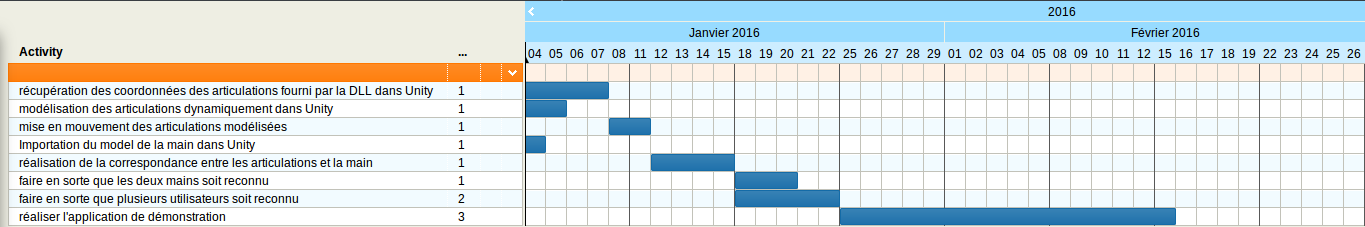
\includegraphics[angle=-90, width=4cm]{images/planning.png}
    \caption{Planning du projet}
    \label{fig:planning}
  \end{center}
\end{figure}
%TODO expliquer quel sera la demo de fin
